\documentclass[UTF8,a4paper,12pt]{ctexart}
\usepackage[margin=2.2cm]{geometry}
\usepackage{graphicx}
\usepackage{booktabs}
\usepackage{tabularx}
\usepackage{array}
\usepackage{hyperref}
\usepackage{float}
\usepackage{listings}
\usepackage{seqsplit}
\hypersetup{colorlinks=true,linkcolor=blue,urlcolor=blue}
\lstset{basicstyle=\ttfamily\small,breaklines=true,frame=single}
\emergencystretch=3em
\title{实验一：目标检测与识别实验报告}
\author{姓名：\underline{\hspace{4cm}}\\ 学号：\underline{\hspace{4cm}}}
\date{2026年8月}
\begin{document}
\maketitle

\begin{abstract}
本实验面向鼠标、笔记本电脑、水杯和手机四类桌面物体，完成了数据采集、ISAT标注、YOLO格式转换、YOLOv8n迁移学习以及Jetson Orin部署。模型在Jetson上通过USB摄像头进行推理，并实时显示类别、检测框、置信度、物体数量和FPS。在具有时间相关性的帧级诊断集上，模型正确匹配104个标注目标中的103个，精确率为100.00\%，召回率（对象级诊断准确率）为99.04\%。Jetson演示画面中可同时检测多个类别，并显示15.0 FPS。上述结果证明了原型系统可运行，但课程要求的独立20个实物准确率、稳定平均FPS和ROS2端到端运行记录仍需补充，不能提前将帧级诊断结果写成最终验收准确率。
\end{abstract}

\section{实验目的与验收要求}
实验目标为：（1）同时检测不少于两类桌面物体；（2）使用自行采集和标注的数据训练目标检测模型；（3）在Jetson上部署和运行模型；（4）实时显示类别、检测框、置信度和帧率；（5）通过ROS2发布识别结果。课程验收要求包括：至少识别两类物体；测试不少于20个物体且准确率不低于80\%；Jetson实时速度不低于5 FPS；保存测试结果和典型错误案例。

\section{硬件与软件环境}
\begin{table}[H]\centering\caption{实验环境}\begin{tabularx}{\textwidth}{lX}\toprule 项目 & 配置 \\\midrule
训练计算机 & Windows 11；显卡和CUDA信息请根据训练电脑实际配置补充。\\
嵌入式平台 & Jetson Orin，aarch64，Ubuntu 20.04.6，L4T R35.6.4 / JetPack 5.1.6。\\
GPU软件 & CUDA 11.4；NVIDIA PyTorch 2.0.0a0；torchvision 0.15.1，CUDA NMS测试正常。\\
Python与框架 & Jetson端Python 3.8；Ultralytics 8.4.22；YOLOv8n。\\
摄像头 & USB摄像头，输入分辨率640$\times$480；具体型号：\underline{\hspace{3cm}}。\\
ROS2 & 使用rclpy、cv\_bridge、sensor\_msgs和vision\_msgs；发行版：\underline{\hspace{2cm}}。\\
\bottomrule\end{tabularx}\end{table}

\section{数据集与标注}
数据集由自行录制的视频抽帧得到，共595张图片，包含mouse、laptop、cup和phone四个类别。原始标注采用ISAT多边形格式，转换程序根据多边形重新计算外接矩形，归一化坐标后生成YOLO标注，同时检查越界框、删除近重复框并保存数据来源清单。

\begin{table}[H]\centering\caption{数据集划分与目标数量}\begin{tabular}{lrrr}\toprule 划分 & 图片数 & 目标数 & mouse/laptop/cup/phone\\\midrule
训练集 & 421 & 506 & 119/85/212/90\\
验证集 & 87 & 104 & 28/17/42/17\\
测试诊断集 & 87 & 104 & 28/17/42/17\\\bottomrule\end{tabular}\end{table}

数据按照19个来源组内部的连续时间块划分，避免完全随机打散相邻视频帧。但是同一来源组仍出现在三个划分中，因此测试帧与训练帧存在相关性，测试诊断结果不能替代独立实物测试。

\section{方法与训练设置}
以COCO预训练YOLOv8n为初始模型，迁移学习得到四分类检测器。训练100轮，输入尺寸640，batch size为16，使用GPU 0，数据加载线程数为0，随机种子为42，优化器采用Ultralytics自动选择，使用标准YOLO数据增强，早停耐心值为25。训练只使用训练集和验证集，测试诊断集不参与优化。

\begin{lstlisting}[caption={模型训练命令}]
python train_yolo.py --epochs 100 --batch 16 --device 0 --workers 0
\end{lstlisting}

\section{训练与帧级诊断结果}
验证集上记录到的最高mAP@0.5:0.95为0.98571，出现在第76轮。第100轮时Precision为0.99417，Recall为0.99405，mAP@0.5为0.99104，mAP@0.5:0.95为0.98078。完整训练曲线和混淆矩阵保存在\texttt{training/yolov8n\_4class\_finetune/}目录。

\begin{figure}[H]\centering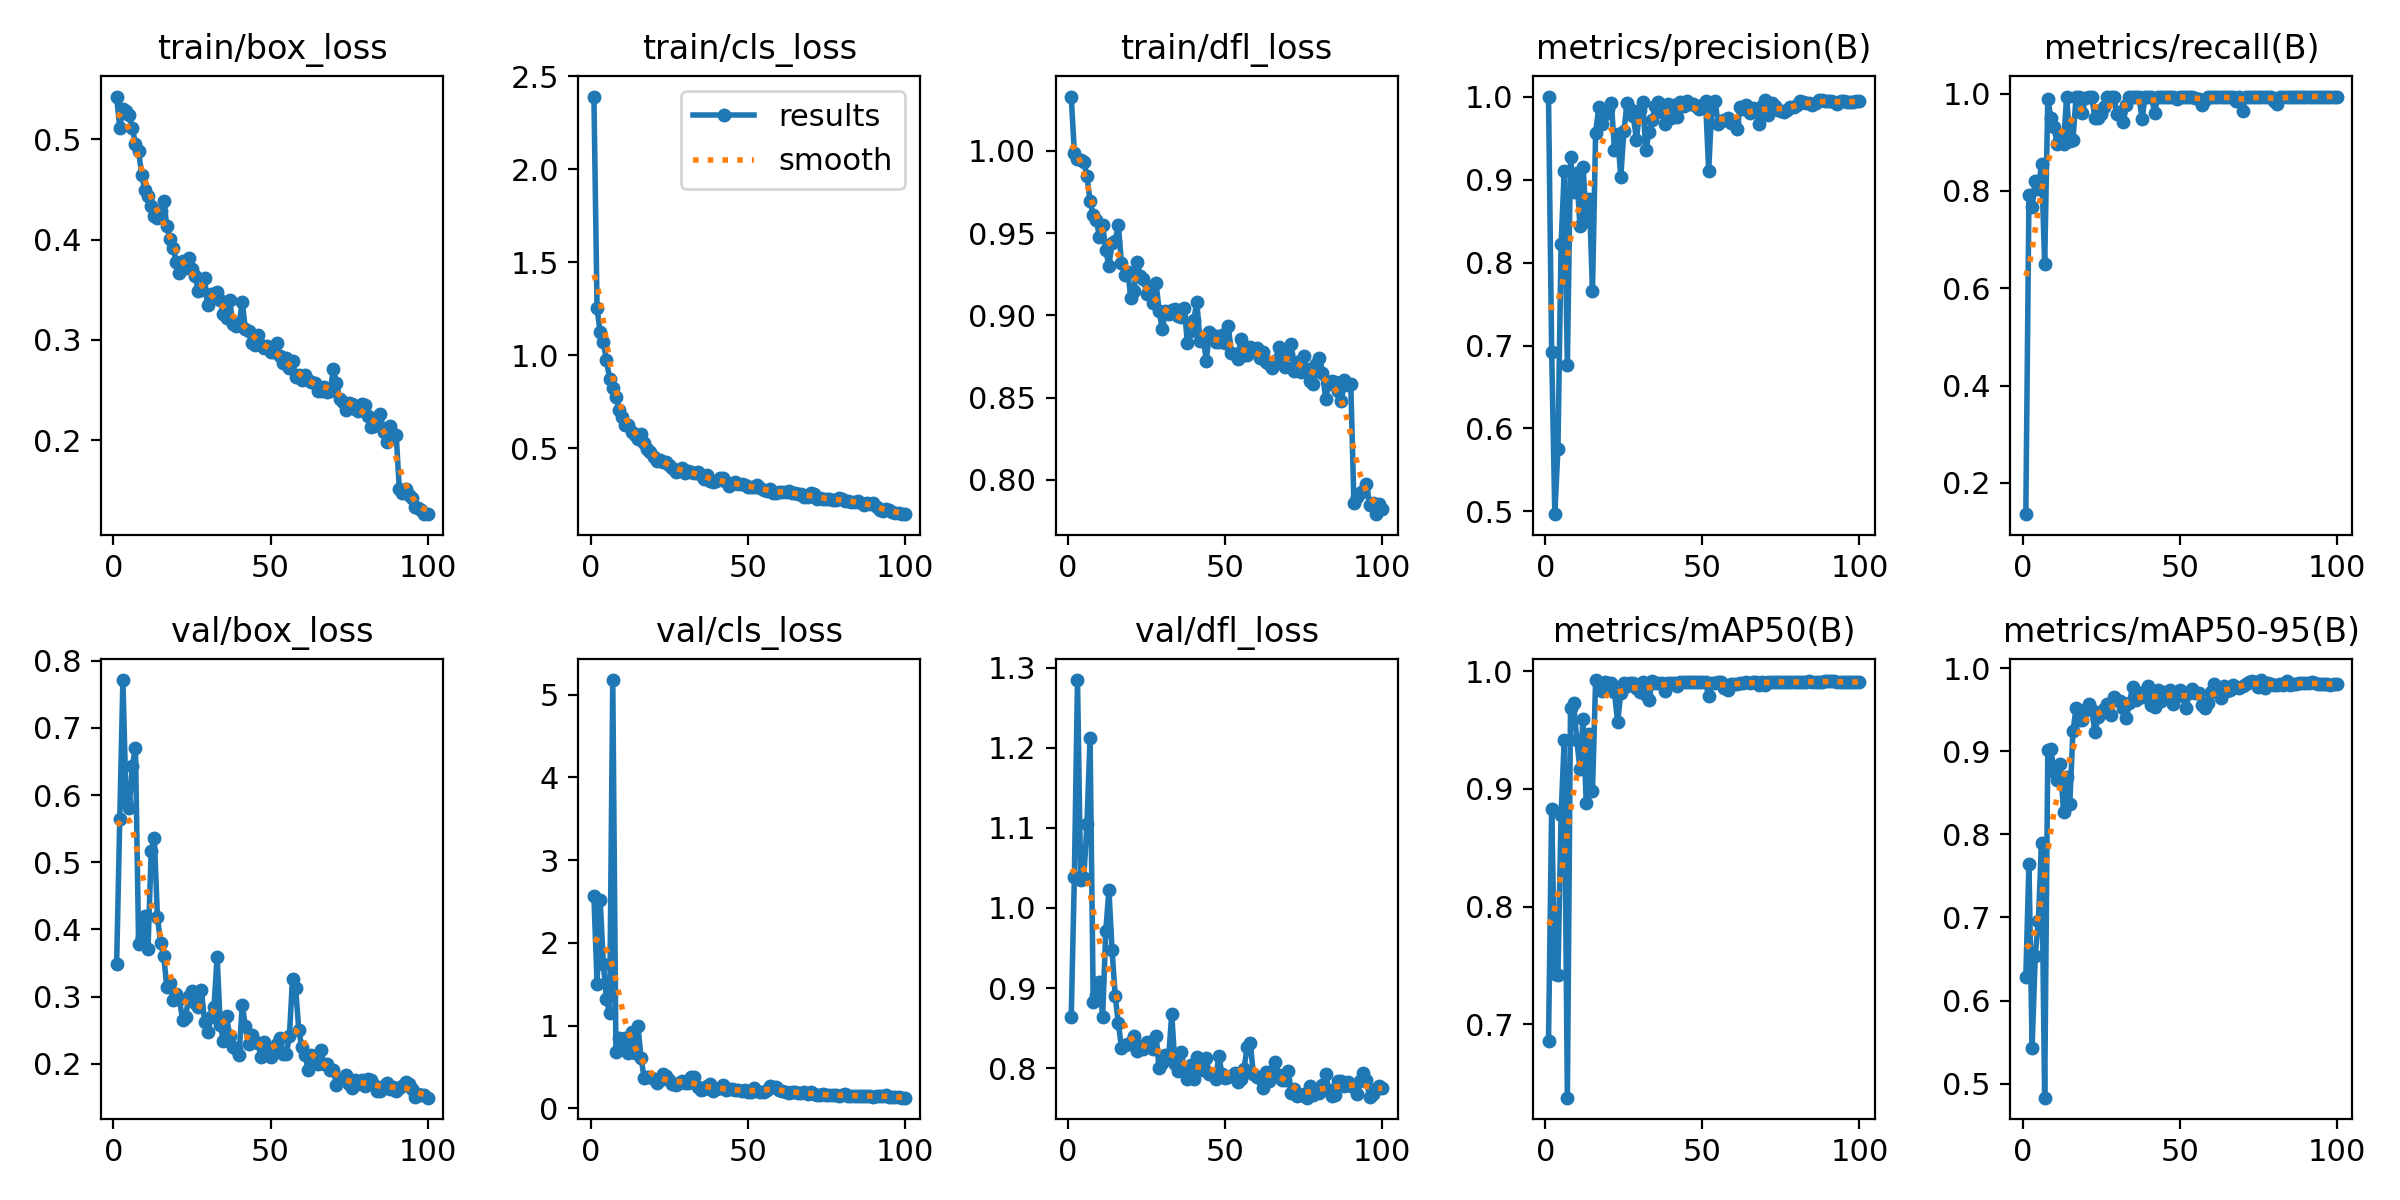
\includegraphics[width=0.98\textwidth]{../training/yolov8n_4class_finetune/results.png}\caption{100轮训练损失和验证指标曲线。曲线显示模型逐渐收敛并在后期趋于稳定。由于只有一次训练，无法估计不同随机种子之间的波动。}\label{fig:trainingzh}\end{figure}

在置信度阈值0.25、匹配IoU阈值0.50下，104个标注目标中有103个被正确匹配，漏检1个，误检0个。

\begin{table}[H]\centering\caption{帧级诊断分类型结果}\begin{tabular}{lrrrr}\toprule 类别 & 标注数 & 正确数 & 漏检数 & 召回率 \\\midrule
mouse & 28 & 28 & 0 & 100.00\%\\
laptop & 17 & 17 & 0 & 100.00\%\\
cup & 42 & 41 & 1 & 97.62\%\\
phone & 17 & 17 & 0 & 100.00\%\\
总计 & 104 & 103 & 1 & 99.04\%\\\bottomrule\end{tabular}\end{table}

\begin{figure}[H]\centering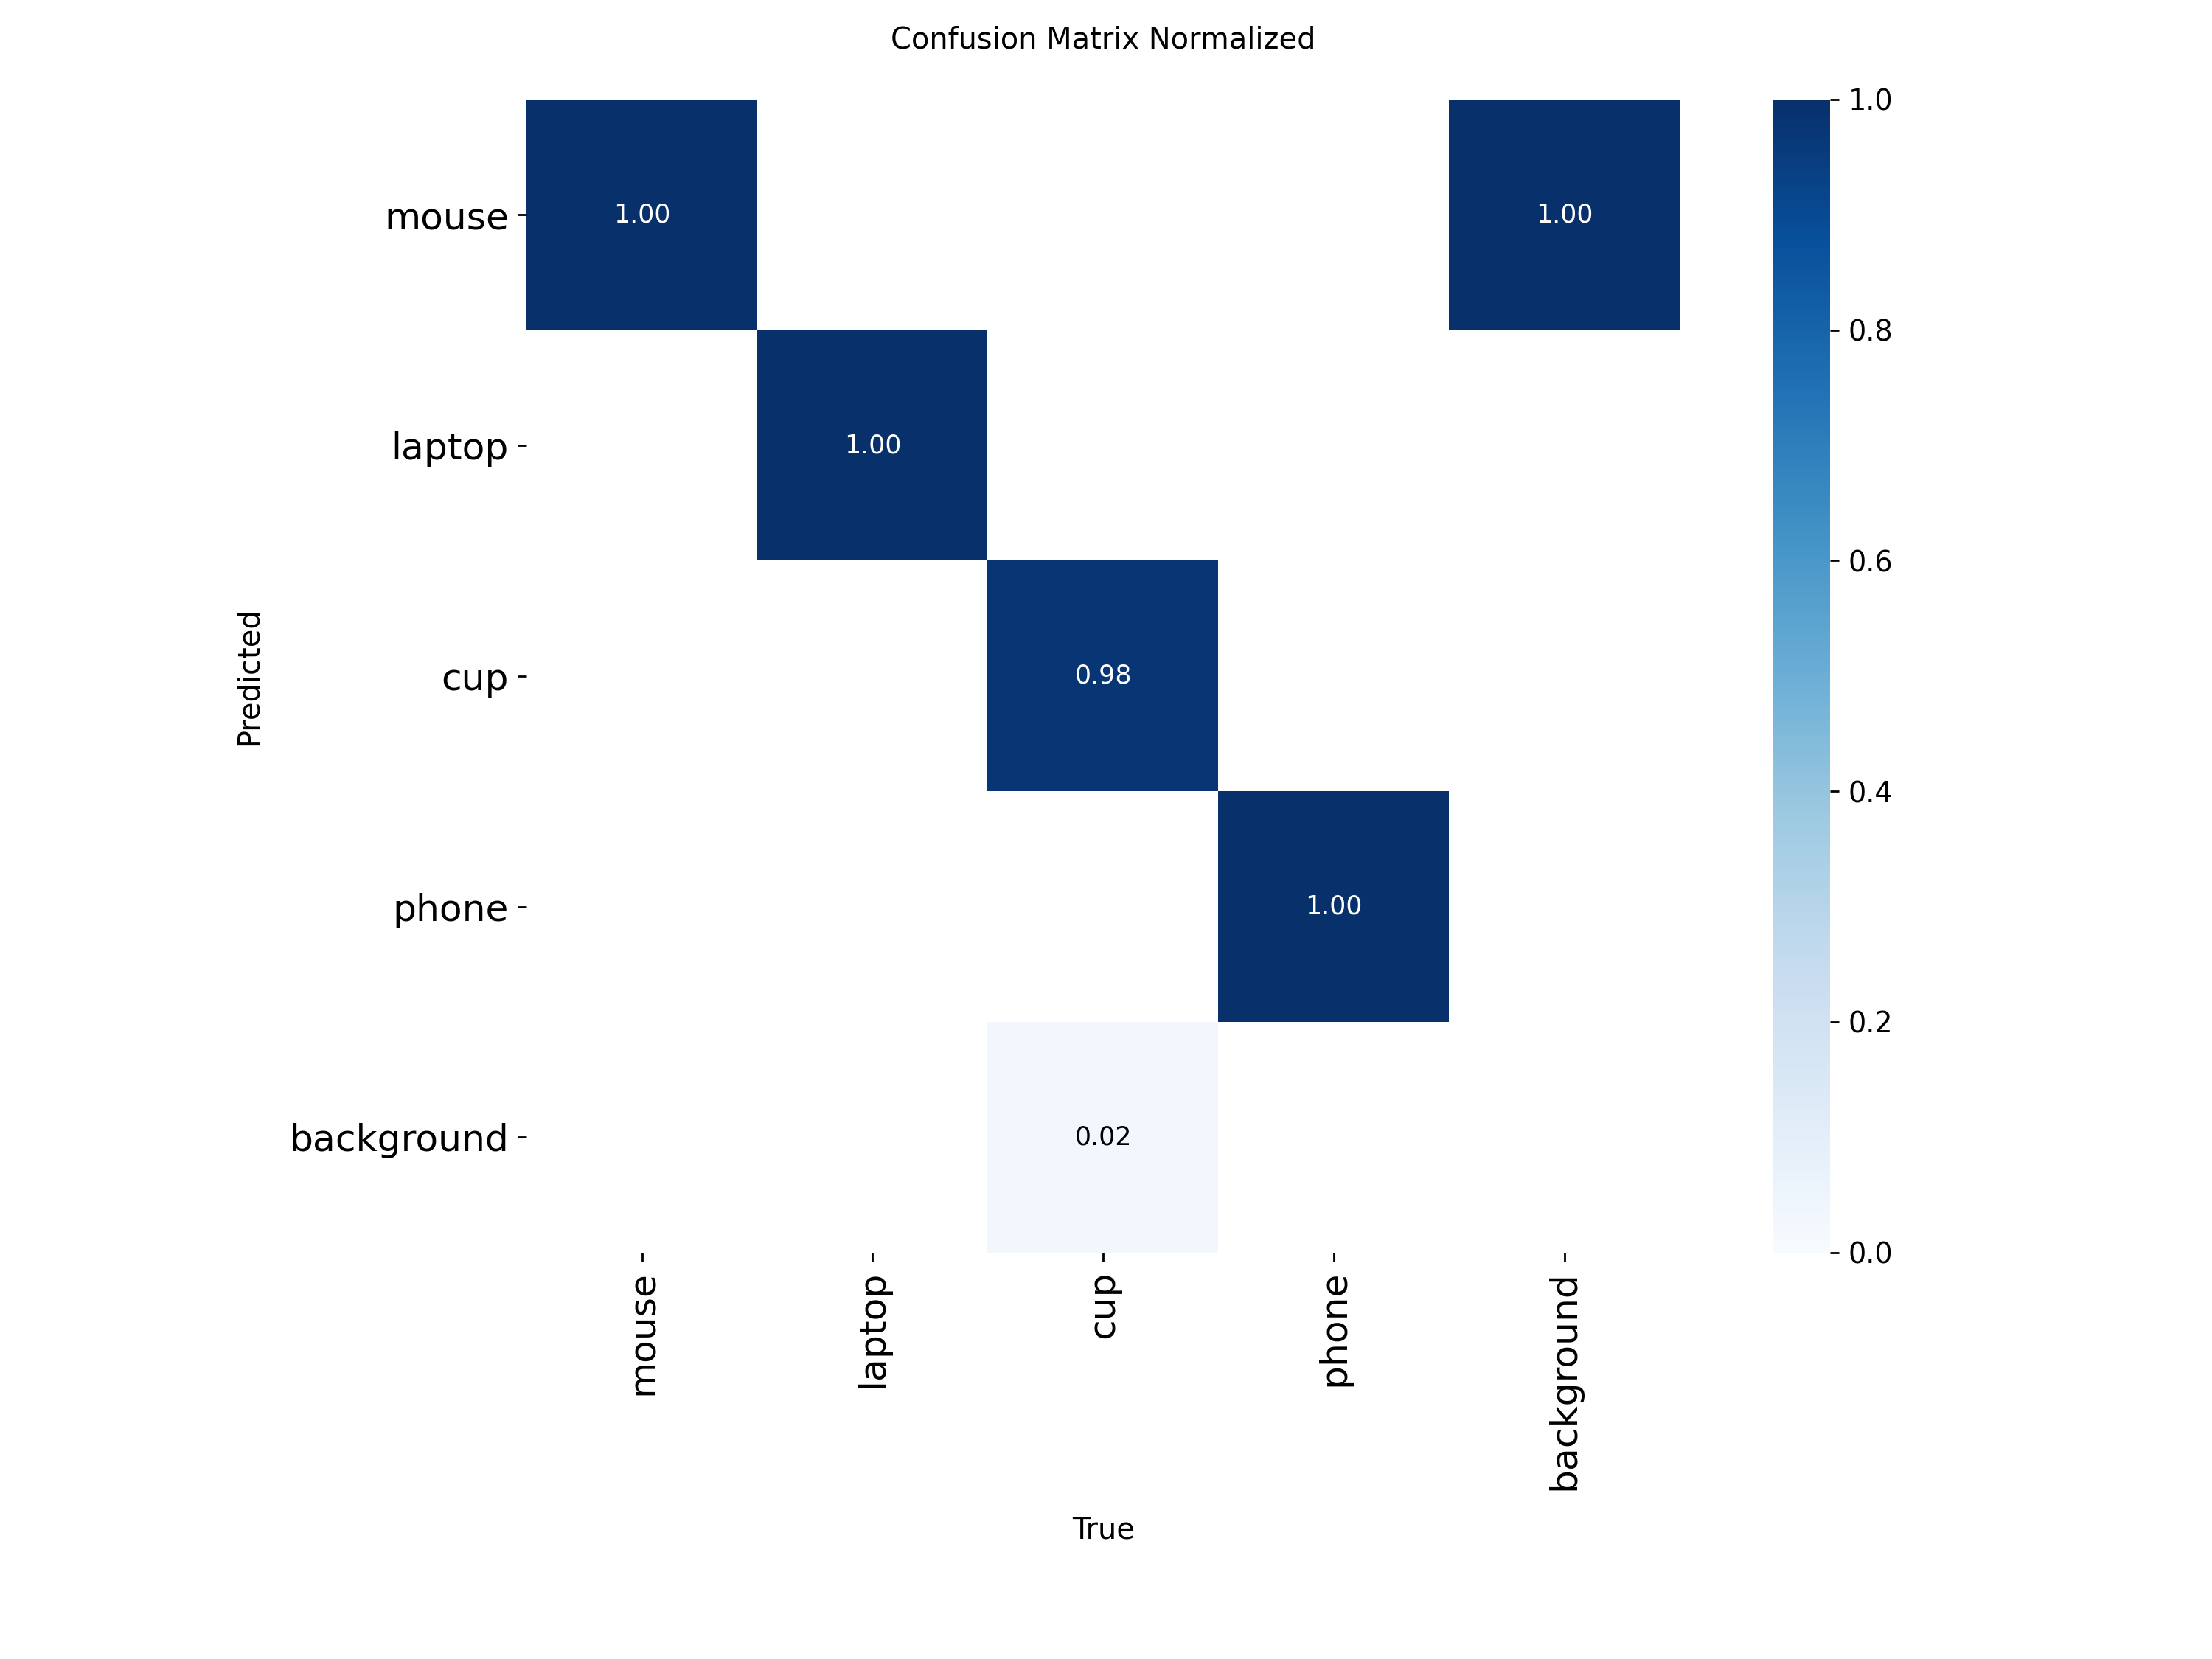
\includegraphics[width=0.75\textwidth]{../training/yolov8n_4class_finetune/confusion_matrix_normalized.png}\caption{归一化验证集混淆矩阵。对角线占主导，说明验证帧上的类别混淆较少。}\label{fig:cmzh}\end{figure}

99.04\%仅表示帧级诊断结果。由于相邻帧和来源组存在相关性，不能将该数值直接写成最终现实物体识别准确率。

\section{Jetson部署与实时检测}
通过部署脚本将\texttt{weights/best.pt}复制到Jetson，使用\texttt{realtime\_detect.py}加载模型。程序使用V4L2打开USB摄像头，使用GPU推理，绘制检测框和置信度，统计各类别物体数量，计算滑动窗口FPS，并支持保存带标注的MP4视频。

\begin{lstlisting}[caption={Jetson实时检测命令}]
python realtime_detect.py --weights ~/robotics_exp1/weights/best.pt \\
  --source 0 --imgsz 320 --confidence 0.35 --device 0 \\
  --camera-width 640 --camera-height 480 --camera-fps 30 \\
  --output ~/robotics_exp1/results/demo.mp4
\end{lstlisting}

\begin{figure}[H]\centering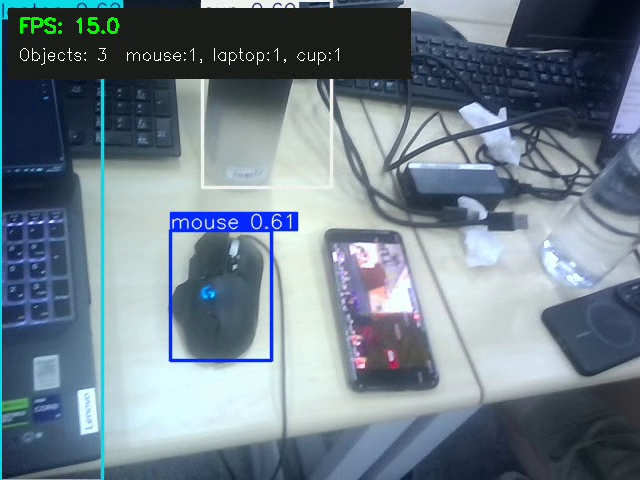
\includegraphics[width=0.9\textwidth]{figures/jetson_demo_frame.jpg}\caption{Jetson实时检测演示画面。画面同时识别出mouse、laptop和cup，显示检测框、置信度、物体数量以及15.0 FPS。该15.0 FPS是画面中的滑动窗口观测值，不是保存的长时间平均速度。}\label{fig:jetsonzh}\end{figure}

演示视频保存在\texttt{results/jetson\_demo.mp4}。最终提交前，应连续运行30--60秒并补充平均和最低FPS：\textbf{平均FPS = \underline{\hspace{2cm}}；最低FPS = \underline{\hspace{2cm}}；平均值是否达到5 FPS：\underline{\hspace{1.5cm}}}。

\section{ROS2结果发布}
\texttt{ros2\_detector\_node.py}订阅\texttt{/camera/image\_raw}图像话题（\texttt{sensor\_msgs/Image}），通过\texttt{cv\_bridge}转换图像并进行YOLO推理，然后向\texttt{/detections}发布\texttt{vision\_msgs/Detection2DArray}。每个检测结果包含像素坐标下的中心点、宽度、高度、类别名称和置信度。

\begin{lstlisting}[caption={ROS2验证命令}]
python ros2_detector_node.py --weights ~/robotics_exp1/weights/best.pt \\
  --image-topic /camera/image_raw --output-topic /detections --device 0
ros2 topic echo /detections --once
\end{lstlisting}

当前项目包含ROS2实现代码，但尚未归档端到端运行截图或话题记录。此处应补充终端截图或rosbag记录：\textbf{ROS2证据：\underline{\hspace{7cm}}}。

\section{独立20个实物测试}
准确率必须使用至少20个彼此独立的实物进行测试，而不能使用相邻视频帧代替。测试结果填写在\texttt{results/independent\_test\_template.csv}中。

\begin{table}[H]\centering\caption{独立实物验收测试（待填写）}\begin{tabular}{lrrr}\toprule 类别 & 测试数 & 正确数 & 准确率 \\\midrule
mouse & \underline{\hspace{1cm}} & \underline{\hspace{1cm}} & \underline{\hspace{1cm}}\\ laptop & \underline{\hspace{1cm}} & \underline{\hspace{1cm}} & \underline{\hspace{1cm}}\\ cup & \underline{\hspace{1cm}} & \underline{\hspace{1cm}} & \underline{\hspace{1cm}}\\ phone & \underline{\hspace{1cm}} & \underline{\hspace{1cm}} & \underline{\hspace{1cm}}\\\midrule 总计 & \underline{\hspace{1cm}} & \underline{\hspace{1cm}} & \underline{\hspace{1cm}}\\\bottomrule\end{tabular}\end{table}

准确率的计算方式为“正确识别物体数除以测试物体总数，再乘以100\%”。如果测试20个物体，至少需要正确识别16个才能达到80\%。

\section{典型错误与改进}
\texttt{results/yolov8n\_4class\_finetune\_test/errors/cup\_cup4\_000086.jpg}保存了帧级诊断中的唯一漏检案例。水杯具有反光、视角变化、局部遮挡和背景相似等问题，容易造成外观特征不稳定。后续可增加不同视角和光照的数据，扩充背景类型，平衡各来源组，复核标注一致性，并在独立验证集上调节置信度阈值。

\section{结论}
本实验完成了四类桌面物体YOLOv8n检测器的训练和Jetson部署，并实现了实时框选、类别显示、置信度显示、物体计数和视频保存。帧级诊断结果为103/104，召回率（对象级诊断准确率）99.04\%，仅有一个cup漏检；Jetson演示画面显示15.0 FPS。项目还实现了ROS2\texttt{Detection2DArray}发布节点。当前最可靠的结论是系统原型已经能够运行；在补充独立20个实物测试、稳定平均FPS和ROS2话题证据之前，不应宣称最终验收已经全部通过。

\section*{复现材料索引}
\begin{itemize}
\item 数据集配置：\path{dataset/yolo/data.yaml}；转换摘要：\path{dataset/yolo/conversion_summary.json}。
\item 最终权重：\path{weights/best.pt}；SHA-256：\texttt{\seqsplit{595C8FD32BE2A733BF0845A5FC89847DAD425A1FDEC249C0375E0DEA9B9CFBA5}}。
\item 训练指标：\path{training/yolov8n_4class_finetune/results.csv}及相关曲线。
\item 评估结果：\path{results/yolov8n_4class_finetune_test/summary.json}和\path{per_image.csv}。
\item 部署与ROS2源码：\path{jetson_setup/deploy_to_jetson.ps1}、\path{realtime_detect.py}、\path{ros2_detector_node.py}。
\item 演示视频：\texttt{results/jetson\_demo.mp4}。
\end{itemize}
\end{document}
